\documentclass{article}
\usepackage{graphicx,fancyhdr,amsmath,amssymb,amsthm,subfig,url,hyperref}
\usepackage[margin=1in]{geometry}
\usepackage{xltxtra}
\usepackage{xgreek}
\usepackage{amsfonts}
\usepackage{amssymb}
\usepackage{amsmath}
\usepackage{graphicx}
\usepackage{listings}
\usepackage{framed}

\usepackage{caption}
\usepackage{ subfig}
%\setmainfont[Mapping=tex-text]{Times New Roman}
\setmainfont{GFS Artemisia}
%----------------------- Macros and Definitions --------------------------
% FILL THIS OUT
\newcommand{\studentname}{Νικόλαος Ζαρίφης}
\newcommand{\suid}{03112178}
\newcommand{\exerciseset}{Τέταρτη εργαστηριακή Άσκηση}
% END



\renewcommand{\theenumi}{\bf \Alph{enumi}}

%\theoremstyle{plain}
%\newtheorem{theorem}{Theorem}
%\newtheorem{lemma}[theorem]{Lemma}

\fancypagestyle{plain}{}
\pagestyle{fancy}
\fancyhf{}
\fancyhead[RO,LE]{\bfseries\large NTUAthens}
\fancyhead[LO,RE]{\bfseries\large Δίκτυα επικοινωνιών}
\fancyfoot[LO,RE]{\bfseries\large \studentname: nick.zarifis@hotmail.com}
\fancyfoot[RO,LE]{\bfseries\thepage}
\renewcommand{\headrulewidth}{1pt}
\renewcommand{\footrulewidth}{1pt}

\graphicspath{{figures/}}

%-------------------------------- Title ----------------------------------

\title{Δίκτυα επικοινωνιών \\ \exerciseset}
\author{\studentname \qquad  ID: \suid}

%--------------------------------- Text ----------------------------------

\begin{document}
\maketitle
\begin{figure}[ht!]
	\centering
	\subfloat[nam]{{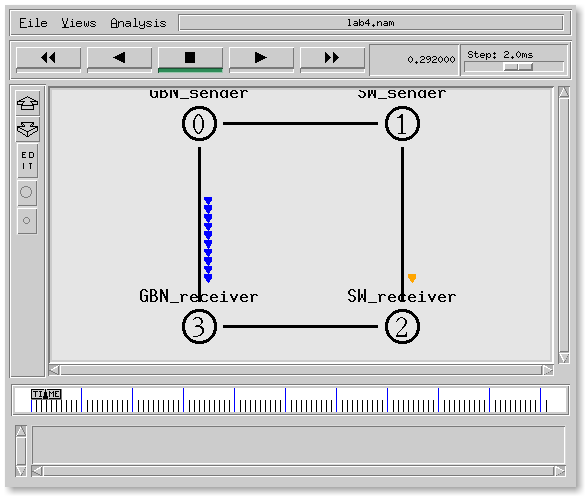
\includegraphics[height=70pt,width=70pt]{nam}}
	}
	\qquad
	
\end{figure}

\section*{Ερωτήσεις 1}
\begin{itemize}
	\item \textbf{Με τη βοήθεια του NAM, εντοπίστε τη χρονική στιγμή που ολοκληρώνεται η μετάδοση των 100
		πακέτων FTP στην περίπτωση του πρωτοκόλλου: (i) Go back N και (ii) Stop and Wait}\\
	Σύμφωνα με το nam παρατηρούμε ότι στα 0,87s περίπου του Go back N όπου φτάνει η τελευταία επιβεβαίωση πακέτων στον κόμβο. Σε αντίθεση η Stop and Wait η τελευταία επιβεβαίωση του πακέτου φτάνει στα 10,128s παραπάνω από το δεκαπλάσιο χρόνο!
	\item \textbf{Ποιο είναι το ελάχιστο μέγεθος παραθύρου εκπομπής (Nopt) που εξασφαλίζει ελάχιστο χρόνο
		μετάδοσης του συνόλου των πακέτων στο πρωτόκολλο Go back N;}\\
	Καταρχάς ξέρουμε ότι η ζεύξη έχει εύρος 3Mbs όποτε χρησιμοποιώντας τον γνωστό τύπο: Ευρως*καθυστέρηση=144000bits=18000B.Άρα τα πακέτα που χωρά είναι: $\frac{18000}{1000}=18$\footnote{960+γιατί προσθέτουμε το επικεφαλίδες,το βλέπουμε κι μέσα στο αρχείο tr} δηλαδή 18 πακέτα.Επίσεις για κάθε πακέτο υπάρχει κι μια επιβεβαίωση .Αρα $w=2BD+1=37$.Το +1 γιατί δεν προκυπτει να σταλεί πλαίσιο μέχρι να παραληφθεί πλήρες ένα πλαίσιο.Πράγμα που μας επιβεβαιώνει το βιβλίο.
	\item \textbf{Με βάση το ελάχιστο αυτό μέγεθος παραθύρου που προσδιορίσατε στο προηγούμενο ερώτημα,
		τροποποιήστε τις εντολές\\
		\$tcp0 set window\_ X \\
		\$tcp0 set windowInit\_ X\\
		εκτελέστε την προσομοίωση και υπολογίστε τη χρονική στιγμή που ολοκληρώνεται η μετάδοση
		των 100 πακέτων FTP για το πρωτόκολλο Go back N με τη βοήθεια του NAM.}\\
	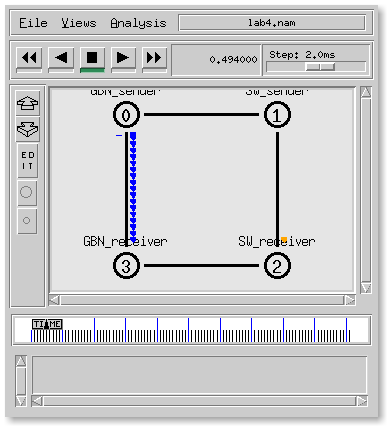
\includegraphics[width=100pt,height=88pt]{nam2} \\
	Βλέπουμε ότι η αποστολή των πακέτων ολοκληρώνεται σε 0,55s. 
	\item \textbf{Πόση είναι η μέγιστη καθυστέρηση διάδοσης της ζεύξης n(0)-n(3) ώστε το αρχικό μέγεθος
				παραθύρου (Ν=10) να οδηγεί σε συνεχή χρησιμοποίηση της ζεύξης (no idle time);}\\ Πρέπει $w=10=2*BD+1=2*18*d+1 \rightarrow d=25ms$. \\
			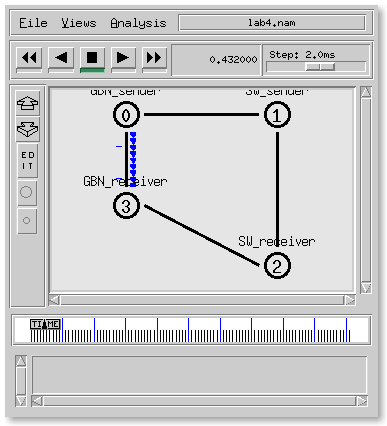
\includegraphics[width=100pt,height=90pt]{nam3} .
			\item \textbf{Εκτελέστε πάλι την προσομοίωση με το μέγεθος παραθύρου του πρωτοκόλλου Go back N που
				βρήκατε στο δεύτερο ερώτημα (Nopt), όταν η ζεύξη n(0)-n(3) έχει διπλάσια και υποτριπλάσια
				καθυστέρηση διάδοσης της αρχικής. Εντοπίστε τη χρονική στιγμή που ολοκληρώνεται η μετάδοση
				των 100 πακέτων FTP στον κόμβο n3 στις δύο αυτές περιπτώσεις. Τι παρατηρείτε;} \\
			\begin{figure}[ht!]
				\centering
				\subfloat[16ms]{{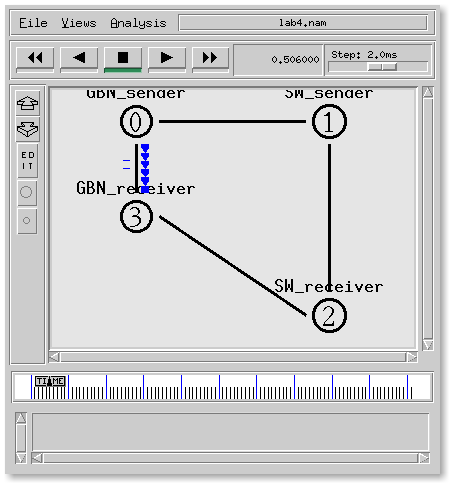
\includegraphics[height=100pt,width=100pt]{naml1}}
				}
				\qquad
				\subfloat[96ms]{{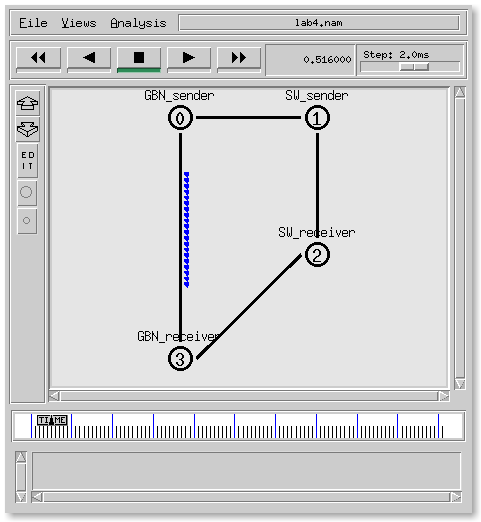
\includegraphics[height=100pt,width=100pt]{naml2}}}
			\end{figure}\\
			Βάζοντας πρώτα στα 16ms βλέπουμε ότι η ροή είναι συνεχόμενη και ότι τελειώνει στα 0.53s.Ενώ στα 96ms βλέπουμε ότι δεν είναι συνεχόμενη και τελειώνει σε 0.804s.Βλέπουμε πως με παραπάνω καθυστέρηση γίνεται πιο αργά η μεταφορά κι δεν αξιοποιήτε πλήρως η γραμμή σε αντίθεση με την μικρή καθυστέρηση.
	\end{itemize}
\section*{Ερωτήσεις 2}
d=178ms
\begin{itemize}
	\item \textbf{Ποιος είναι ο αριθμός των πακέτων που παρελήφθησαν, πόσα δεδομένα παρελήφθησαν από τον
		παραλήπτη κατά τη διάρκεια της προσομοίωσης για κάθε ροή κίνησης;}
	\\Η απάντηση βγαίνει από το αποτέλεσμα του script(τροποποίησα τον χρόνο εκτέλεσης ).
		\begin{framed}
			N=10
			\\Total Data received for flow ID 0	: 99960 Bytes\\
			Total Packets received for flow ID 0	: 100\\
			Last packet received for flow ID 0	: 3.68352 sec\\
			Total Data received for flow ID 1	: 99960 Bytes\\
			Total Packets received for flow ID 1	: 100\\
			Last packet received for flow ID 1	: 35.94912 sec
			 \end{framed}
	\begin{framed}
		Nopt
		\\Total Data received for flow ID 0	: 99960 Bytes\\
		Total Packets received for flow ID 0	: 100\\
		Last packet received for flow ID 0	: 1.214773 sec\\
		Total Data received for flow ID 1	: 99960 Bytes\\
		Total Packets received for flow ID 1	: 100\\
		Last packet received for flow ID 1	: 35.94912 sec\end{framed}
	\item \textbf{Εξετάζοντας το αρχείο ίχνους, προσδιορίστε σε πόσο χρόνο απεστάλησαν αυτά τα δεδομένα στις
		δύο περιπτώσεις για κάθε ροή κίνησης. Ποιος ο μέσος ρυθμός μετάδοσης δεδομένων σε bps και
		ποια είναι η χρησιμοποίηση του καναλιού;}
	\\ Καταρχάς η αποστολή ξεκινάει στα 0.25s. Για \textit{N=10} έχουμε ότι ο χρόνος που έκαναν για να μεταδοθούν τα δεδομένα ήταν για την στο πρωτόκολλο GBN ήταν \textit{3.43352s} ενώ στο SW \textit{35.79912s }.
	Ο μέσος ρυθμός μεταδώσεις είναι:
	Για GBN: $\frac{Data}{time}=\frac{99960*8}{3.43352}=232903,842121205bps$
	Η χρησιμοποίηση είναι:
	$\frac{mean\ rate}{channel\ rate}=\frac{232903,842121205bps}{3Mbs}=0,077634614=7.76 \%$
	\\
	Για  SW:$\frac{Data}{time}=\frac{99960*8}{35.79912}=3573,390315728bps$
	Η χρησιμοποίηση είναι:
	$\frac{mean\ rate}{channel\ rate}=\frac{3573,390315728bps}{3Mbs}=0.001=0.1 \%$\\
	Για \textit{N=37} ο χρόνος μετάδωσεις είναι για το GBN:0.964773s .To SW δεν αλλάζει εδώ.
		Ο μέσος ρυθμός μεταδώσεις είναι:
		Για GBN: $\frac{Data}{time}=\frac{99960*8}{0.964773}=828878,917631401bps$
		Η χρησιμοποίηση είναι:
		$\frac{mean\ rate}{channel\ rate}=\frac{828878,917631401bps}{3Mbs}=0,276292973=27,6 \%$
		\\
	\item \textbf{Τροποποιείστε το script ώστε να υπολογίσετε το χρόνο λήψης της επιβεβαίωσης (τύπος πακέτου
		ack) του τελευταίου πακέτου στις δύο περιπτώσεις για κάθε ροή κίνησης. Επισυνάψτε στην
		απάντησή σας και το τροποποιημένο script.}\\
	\begin{framed}/r$\hat{}$/\&\&/ack/ \{
		
		flow\_id = \$8;\\
		if (flow\_id == 0) \{\\
			last\_0= \$2;\\
		\}
		if (flow\_id == 1) \{\\
			last\_1= \$2;\\
		\}\}
	\end{framed}
		Τρέχοντας έχουμε το ακόλουθο αποτέλεσμα:N=10\begin{framed}Last ack packet on flow ID 1	: 3.861627 sec\\
			Last ack packet on flow ID 2	: 36.127227 sec
			\end{framed}
			Και για N=37:\begin{framed}Last ack packet on flow ID 1	:1.39288 sec
				\\
				Last ack packet on flow ID 2	: 36.127227 sec
			\end{framed}
\end{itemize}
\end{document}